\chapter{Proposed Personalized Node-DP Mechanism}\label{ch:method}
Figure~\ref{fig:pdp-workflow} shows how the public Registry informs one-time participation, how the retained graph supports slot-local training, and how the final model is evaluated on the held-out test graph. The workflow uses the GRAT3 model and RWR/SCS/BES sampling inherited from PrivIM \cite{hou2025}.

\begin{figure}[htbp]
\centering
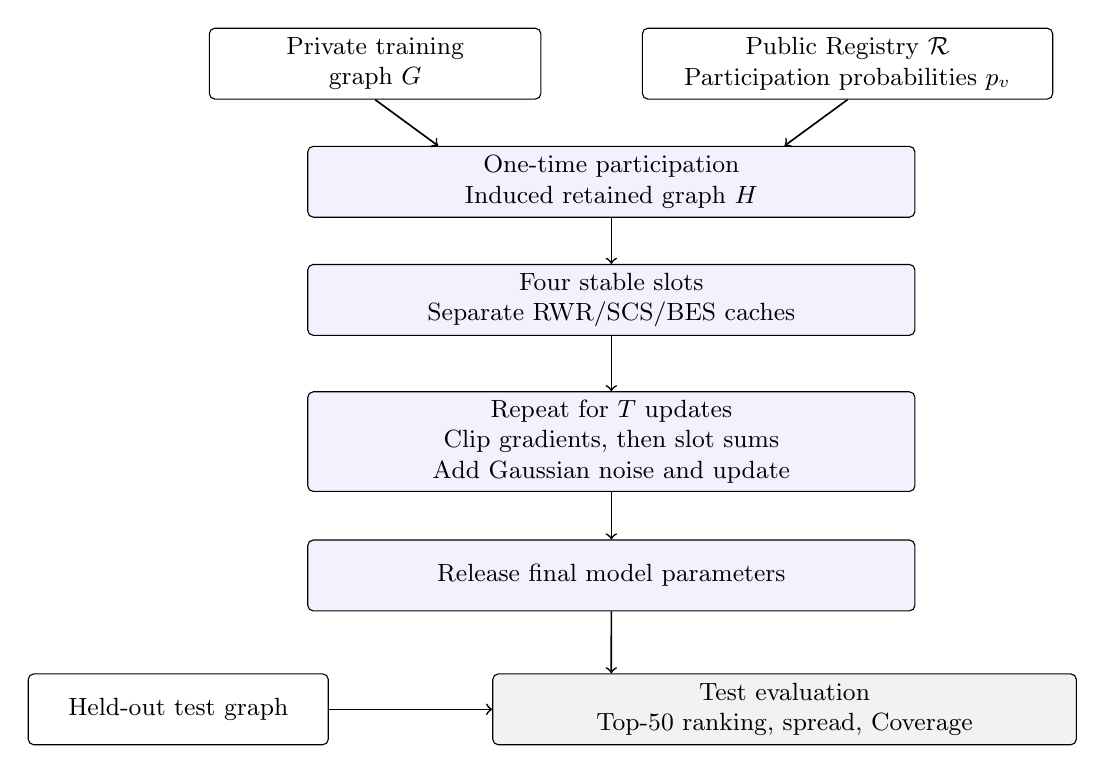
\begin{tikzpicture}[
  font=\small,
  stage/.style={draw, rounded corners=2pt, align=center, minimum height=9mm,
                inner sep=3pt, fill=blue!5},
  input/.style={stage, fill=white},
  eval/.style={stage, fill=black!5},
  flow/.style={->, semithick},
  x=1mm, y=1mm
]
\node[input, text width=40mm] (graph) at (-30,0) {Private training\\graph \(G\)};
\node[input, text width=50mm] (registry) at (30,0) {Public Registry \(\mathcal R\)\\Participation probabilities \(p_v\)};
\node[stage, text width=75mm] (retain) at (0,-15) {One-time participation\\Induced retained graph \(H\)};
\node[stage, text width=75mm] (slots) at (0,-30) {Four stable slots\\Separate RWR/SCS/BES caches};
\node[stage, text width=75mm] (updates) at (0,-48) {Repeat for \(T\) updates\\Clip gradients, then slot sums\\Add Gaussian noise and update};
\node[stage, text width=75mm] (model) at (0,-65) {Release final model parameters};
\node[input, text width=36mm] (test) at (-55,-82) {Held-out test graph};
\node[eval, text width=72mm] (evaluation) at (22,-82) {Test evaluation\\Top-50 ranking, spread, Coverage};

\draw[flow] (graph.south) -- ([xshift=-22mm]retain.north);
\draw[flow] (registry.south) -- ([xshift=22mm]retain.north);
\draw[flow] (retain) -- (slots);
\draw[flow] (slots) -- (updates);
\draw[flow] (updates) -- (model);
\draw[flow] (model.south) -- ([xshift=-22mm]evaluation.north);
\draw[flow] (test) -- (evaluation);
\end{tikzpicture}

\caption[PDP-PrivIM training and evaluation workflow]{PDP-PrivIM training and evaluation workflow. The training mechanism releases the final model parameters and genuinely public configuration. Test evaluation combines the model with a separate held-out graph.}
\label{fig:pdp-workflow}
\end{figure}

\section{Frozen system and model}
PDP-PrivIM changes the private training organization while preserving the existing GRAT3, loss, and subgraph construction. The trained parameter vector has dimension 2340. Its three layers map 32 to 32, 32 to 32, and 32 to 1 dimensions, using all-one 32-dimensional input features.

For one layer, let $h_u$ be the input feature vector at node $u$, and let $N^+(u)$ and $N^-(u)$ denote its outgoing and incoming neighbors in the graph supplied to the layer. For each edge $(u,v)$, the released implementation scores the concatenated input features and normalizes over the outgoing edges of $u$. It then aggregates incoming messages at $v$ and applies an affine feature map:
\begin{align}
 e_{uv} &= \operatorname{ReLU}\bigl(a^\top[h_u\Vert h_v]+c\bigr), \\
 \alpha_{uv} &= \frac{\exp(e_{uv})}{\sum_{w\in N^+(u)}\exp(e_{uw})}, \\
 z_v &= W\left(\sum_{u\in N^-(v)}\alpha_{uv}h_u\right)+b .
\end{align}
Here $[h_u\Vert h_v]$ denotes concatenation, $(a,c)$ are the attention weights and scalar bias, and $(W,b)$ are the feature-map weights and bias. An empty incoming sum gives a zero aggregate. The first two layers pass $z_v$ through ReLU before the next layer. The third layer produces the scalar logit, which enters the loss through a sigmoid and is used directly for test ranking.

This parameter count follows directly from the released layer shapes: two layers each contribute $32\cdot32+32+64+1=1121$ coordinates, and the final layer contributes $32+1+64+1=98$, giving $2(1121)+98=2340$. The final projection acts on the 32 weights of the last feature map. Its bias and attention parameters are separate coordinates.

For a sampled subgraph, let $q_i$ be its sigmoid node output and $A^+$ the original adjacency with identity added. The unchanged loss is
\begin{equation}
 \mathcal{L}(q,A^+)=\sum_j\prod_i(1-q_i A^+_{ij})+
 0.5\sum_i q_i.\label{eq:loss}
\end{equation}
The first term penalizes uncovered vertices in the differentiable surrogate; the second penalizes selection mass. The Top-50 training argument does not replace this penalty with a new constrained optimizer. The mathematical description follows the frozen loss implementation rather than proposing a revised objective.

\subsection{What the training surrogate rewards}
On a sampled subgraph, consider an auxiliary seed set in which each node $i$ is selected independently with probability $q_i$. This is a mathematical interpretation of the loss in Equation~\eqref{eq:loss}. The frozen training code evaluates the product directly, and the final evaluator takes the Top-50 scores. Under the auxiliary interpretation, node $j$ is uncovered exactly when every candidate $i$ with $A^+_{ij}=1$ is omitted. Thus
\begin{align}
 \Pr[j\text{ is uncovered}]
 &=\prod_i(1-q_iA^+_{ij}),\\
 \mathcal L(q,A^+)
 &=|V_{\mathrm{sub}}|-\mathbb E[\operatorname{Spread}(S)]
    +0.5\,\mathbb E[|S|],
 \label{eq:expected-surrogate}
\end{align}
where $V_{\mathrm{sub}}$ is the local subgraph vertex set and $S$ in the expectation is the auxiliary seed set. The added identity matrix counts every seed as covered. The product represents one-step spread on the sampled subgraph, with the orientation inherited from the frozen adjacency.

Differentiating with respect to one score gives
\begin{equation}
 \frac{\partial \mathcal L}{\partial q_i}
 =0.5-
   \sum_{j:A^+_{ij}=1}\;\prod_{\ell\ne i}(1-q_\ell A^+_{\ell j}).
 \label{eq:surrogate-derivative}
\end{equation}
The sum is the expected additional reach of seed $i$ under the other candidates' auxiliary probabilities. When another likely seed already covers $j$, the factor for that seed is small, and $j$ contributes less to the benefit of increasing $q_i$. This is how the loss represents neighborhood overlap. For a sigmoid logit $z_i$, the derivative with respect to $z_i$ multiplies Equation~\eqref{eq:surrogate-derivative} by $q_i(1-q_i)$, so the gradient can be small near either endpoint even when the expected marginal reach differs from the selection penalty.

Equations~\eqref{eq:expected-surrogate} and~\eqref{eq:surrogate-derivative} distinguish two training and evaluation decisions. The penalty controls expected selection mass locally during training, while the evaluator imposes a fixed cardinality on a separate graph. In addition, $\operatorname{Spread}$ on the sampled subgraph uses only edges visible in that subgraph. Neighboring vertices outside it can contribute to the test objective but cannot contribute to this gradient. These properties explain why cache construction, model scoring, and the discrete ranking must all be specified to interpret the reported utility.

\section{Public Registry and one-time participation}
The Registry fixes targets for all identities in $U$ before graph training. Its nominal public proportions are 20\%, 40\%, and 40\% for targets 1, 2, and 4, with integer quotas resolved by the existing rule. Those proportions concern the full public universe, not realized training membership or a secret retained graph.

Following the personalized subsampling principle of Jorgensen et al. \cite{jorgensen2015}, the mechanism sets participation probabilities from the public target budgets. For every present identity, it independently draws one Bernoulli decision with probability
\begin{equation}
 p_v=\min\left\{1,\frac{\exp(\epsilon^{\mathrm{tar}}_v)-1}{\exp(2)-1}\right\}.\label{eq:participation}
\end{equation}
The induced retained graph $H$ contains retained nodes and edges between them. Strict identities participate with probability approximately 0.26894142137, while targets 2 and 4 participate with probability one. Sampling occurs once before the complete training run, rather than once per update. The retained set is an internal input, not a released statistic.

\section{Stable slots and local sampling}
Four overlapping identity sets $U_0,\ldots,U_3$ are defined using two public hash partitions. At each of two levels, every identity enters one of two slots. Therefore every identity belongs to exactly $K=2$ slots. Slot membership depends on stable public identity and the frozen hash rule; removing a private node does not rebalance other identities.

Slot $j$ accesses only $H[V(H)\cap U_j]$. It has its own deterministic sampling role stream, batch stream, node mapping, frequency state, subgraph cache, and cursor. The original RWR/SCS/BES sampler runs locally with public subgraph size $n$ and SCS threshold $M$. The reference configuration uses $n=40$, $M=4$, walk length 200, restart probability 0.3, frequency decay 1, BES divisor 2, and $Q=64$ per slot. The rate is $\min\{1,64/\max(1,|V_j|)\}$, used to construct that local cache.

Every update obtains up to four positions from each slot's cache, padding missing positions with zero contribution. There is no borrowing from other slots. Four slots and four positions produce a fixed denominator $B=16$. Cache reuse across updates is allowed because the proof handles arbitrary private within-slot state rather than treating every sampled subgraph as an independent protected record.

\subsection{Role of the inherited sampling stages}
The PrivIM framework organizes subgraph extraction, private training, and accounting as distinct computations \cite{hou2025}. Random Walk with Restart builds training examples around starting vertices. A walk preferentially sees graph paths accessible from its current vertex and periodically returns to its start. Sensitivity-Constrained Sampling (SCS) tracks how often nodes have entered accepted subgraphs. Its frequency-dependent rule limits repeated use of the same vertices. Boundary-Enhanced Sampling (BES) uses the remaining allowances to include structure that the first stage may have missed. In PDP-PrivIM both stages read and update the state for one slot at a time.

The order of these operations matters. Outer participation decides which vertices and incident edges exist in the retained graph for all subsequent updates. Slot membership then determines which retained nodes and edges a sampler can access. Only after those steps can RWR, SCS, and BES form training examples. For instance, having spare allowance in BES can make a vertex eligible for an additional subgraph, provided the vertex already lies in the retained slot graph. An edge unavailable in every slot remains unavailable to the sampler no matter how many walks are taken. Table~\ref{tab:sampling-design} traces each decision to the part of the pipeline it controls.

\begin{table}[htbp]
\centering\small
\caption{Participation, locality, and sampling decisions in PDP-PrivIM}
\label{tab:sampling-design}
\begin{tabularx}{\textwidth}{@{}p{.21\textwidth}XX@{}}
\toprule
Operation & Effect on training input & Role in the conditional analysis \\
\midrule
Outer participation & Retains whole identities and induces a graph for the complete run. & Provides one law for mixing presence and absence of the protected node. \\
Stable slots & Exposes only the induced graph and local state of each slot. & Bounds the number of slot contributions that can change under node removal. \\
RWR, SCS, and BES & Build and reuse local caches with the public size and frequency settings. & May change arbitrarily within a slot touched by the removed node. \\
Zero padding and slot clipping & Reserve a fixed number of positions and bound each slot sum. & Give a common gradient scale and a bounded contribution before Gaussian noise. \\
\bottomrule
\end{tabularx}
\end{table}

\subsection{How participation and local views change structural information}
Some differences in the information available to training can be quantified before a cache is built. For a fixed input graph let $I_v$ indicate whether a present node survives the one-time participation draw. Then $|V(H)|=\sum_{v\in V}I_v$, with expectation $\sum_{v\in V}p_v$. An edge $(u,v)$ with distinct endpoints survives in $H$ exactly when $I_u I_v=1$, giving
\begin{equation}
 \mathbb E[|E(H)|]=\sum_{(u,v)\in E}p_up_v.
 \label{eq:expected-retained-edges}
\end{equation}
The edge indicators need not be independent. For distinct $u,v,w$ with edges $(u,v)$ and $(u,w)$, their covariance is $p_u(1-p_u)p_vp_w$. One strict node's participation decision is shared across all of its incident edges. Its removal can eliminate several paths together, even though the endpoint draws are independent.

Let $c_{uv}=\sum_{j=0}^{3}\mathbf{1}\{u,v\in U_j\}$ count the fixed slots that contain both endpoints. At each of the two partition levels, the endpoints can share at most one slot, so $c_{uv}\in\{0,1,2\}$. The edge has $c_{uv}I_u I_v$ copies across the local graphs. In particular,
\begin{equation}
 \mathbb E\!\left[\sum_{j=0}^{3}|E(H_j)|\right]
 =\sum_{(u,v)\in E}c_{uv}p_up_v .
 \label{eq:expected-slot-edges}
\end{equation}
This sum counts edge copies across slots before cache construction. An edge whose endpoints separate at both levels has no local copy. An edge whose endpoints share a slot at both levels has two copies whenever it survives. A surviving vertex itself occupies exactly two local graphs, including when it is isolated in either one. Node membership and edge visibility are therefore quantified by different expressions.

As an illustration, at the reference participation probability a strict target-1 vertex with two target-2 neighbors retains both incident edges with probability about $0.269$ before slot induction, or loses both with probability about $0.731$. If the two edges have $c_{uv}=0$ and $c_{uw}=2$ respectively, the first edge is absent from every local graph and the second contributes either two copies or none. This calculation uses a hypothetical neighborhood and public parameters. The resulting counts precede the walk, frequency constraints, and optimization, so they cannot determine either the learned ranking or its Coverage.

Group edges by the targets assigned to their two endpoints, ignoring the order of the endpoints for this grouping. Write $p_1=1/(e+1)$ for the participation probability of a target-1 identity. Table~\ref{tab:edge-retention} gives the analytical retention factors for the three types of endpoint pairs induced by the policy. Each factor multiplies the original number of edges of that type when calculating the expected retained count in $H$. For local graphs, it instead multiplies the sum of $c_{uv}$ over that edge class. The public proportions constrain how many identities carry each label, while the edge profile depends on how the graph connects them. Both expectations therefore depend on the endpoints of the actual edges.

\begin{table}[htbp]
\centering\small
\caption{Analytical edge retention factors before local cache construction}
\label{tab:edge-retention}
\begin{tabularx}{\textwidth}{@{}Xcc@{}}
\toprule
Endpoint target classes & $\Pr[(u,v)\in E(H)]$ & Expected local edge copies \\
\midrule
Both targets are 1 & $p_1^2\approx0.0723$ & $c_{uv}p_1^2$ \\
One target is 1, the other is 2 or 4 & $p_1\approx0.2689$ & $c_{uv}p_1$ \\
Both targets are in $\{2,4\}$ & $1$ & $c_{uv}$ \\
\bottomrule
\end{tabularx}
\end{table}

Uniform1 assigns participation probability one to every vertex, so before cache construction it exposes $c_{uv}$ copies of each input edge. This gives a precise structural contrast with PDP-PrivIM while holding the public slot rule fixed. A neighborhood consisting mainly of edges between strict identities has lower marginal edge retention than one connected mainly to targets 2 and 4. The analysis concerns what is available to the learner. It gives no ordering of the eventual training losses: cache construction changes which examples enter, and the two private configurations use different Gaussian scales.

\section{Double clipping and Gaussian update}
Let $g_{tji}\in\R^{2340}$ be the full gradient at update $t$, slot $j$, position $i$. Use the frozen clipping operation, whose real-arithmetic norm bound is 3, to form
\begin{align}
 a_{tji}&=\clip(g_{tji}), &
 b_{tj}&=\clip\left(\sum_{i=1}^{4}a_{tji}\right), &
 S_t&=\sum_{j=0}^{3}b_{tj}.\label{eq:doubleclip}
\end{align}
The implementation includes a $10^{-6}$ denominator offset and inward norm margin. The proof uses the resulting bound rather than claiming that its literal code is identical to an ideal radial clip at every point. Missing positions and predefined nonfinite contributions are replaced by zero. These conventions do not constitute a proof covering every floating-point execution.

For a fixed public update count $T$ and sum-scale noise standard deviation $\sigma_T$, each update adds one Gaussian vector to the aggregate $S_t$ of all four slot contributions. The vectors are drawn independently across updates:
\begin{align}
 Z_t&\sim\mathcal{N}(0,\sigma_T^2I_{2340}), &Y_t&=S_t+Z_t,\\
 \theta_{t+1}&=\Pi\!\left(F\left(\theta_t-\frac{0.005}{16}Y_t\right)\right).
 \label{eq:update}
\end{align}
Here $F$ denotes the specified finite-state repair in the implementation, interpreted only as a function of the noisy state, and $\Pi$ clips the final 32 weights to nonnegative values. The initial model is not projected. There is no momentum, parameter averaging, private stopping decision, or selected intermediate checkpoint. The ideal mechanism performs exactly $T$ updates, including empty-input cases. The PDP-PrivIM reference setting is $T=100$ with $\sigma_{100}=260$.

The Gaussian is full-rank in all 2340 trained coordinates. The update divides both the sum-scale sensitivity and standard deviation by 16, so their ratio is unchanged. In the reference setting, the resulting sensitivity and standard deviation are 0.75 and 16.25. Learning-rate multiplication is further postprocessing.

\begin{algorithm}[H]
\caption{PDP-PrivIM training (ideal mathematical description)}\label{alg:pdp}
\begin{algorithmic}[1]
\Require Legal decoded graph $G$, fixed public $U,\mathcal R$, public initialization seed
\Require Public sampler settings $n,M$, update count $T$, and sum-noise scale $\sigma_T$
\State Draw one independent participation decision per present identity using \eqref{eq:participation}
\State Let $H$ be the induced retained graph; initialize all 2340 GRAT3 coordinates
\For{$j=0,\ldots,3$}
  \State Induce the local graph $H_j = H[V(H)\cap U_j]$
  \State Build slot $j$'s cache from $H_j$ with RWR/SCS/BES using $n,M$
\EndFor
\For{$t=0,\ldots,T-1$}
 \For{$j=0,\ldots,3$}
  \State Read up to four positions using slot $j$'s local cache and cursor
  \State Compute and clip each available full-coordinate loss gradient
  \State Set missing or predefined nonfinite contributions to zero
  \State Clip the sum of the four contributions to obtain $b_{tj}$
 \EndFor
 \State Sum the four slot vectors as $S_t=\sum_{j=0}^{3} b_{tj}$
 \State Draw fresh $Z_t\sim\mathcal N(0,\sigma_T^2I_{2340})$ and set $Y_t=S_t+Z_t$
 \State Update with fixed denominator 16 and learning rate 0.005
 \State Apply original state handling; project only the last 32 feature-map weights
\EndFor
\State \Return Fixed-length final parameters and genuinely public configuration only
\end{algorithmic}
\end{algorithm}

\section{Conditional privacy assumptions}\label{sec:conditions}
The following theorem reconstructs the archived G0 analysis, with Uniform calibrations independently documented in U0 and U2 \cite{projectg0,projectuniform}. Its scope requires three groups of assumptions.

First, $U$, Registry, graph decoder, direction, initialization, and role rules are fixed public auxiliary information. Legal adjacency preserves surviving identities and the auxiliary information. Raw preprocessing and declaring a mapping public are outside this assumption.

Second, all graph-dependent sampling and gradient computations remain slot-local. No global private normalization, cross-slot frequency state, unnoised adaptive scheduler, or private persistent model buffer enters another slot or the update rule. The same noisy transcript determines the same model state on adjacent inputs.

Third, the ideal mechanism uses independent exact Gaussian innovations and the stated participation probabilities; updates and projection depend only on public information and noisy history. The release is the fixed parameter vector, not timing, failure behavior, cache statistics, or unrestricted research diagnostics. Exact continuous arithmetic and distributions are mathematical assumptions rather than certified properties of the machine.

\section{Occurrence-Capped PrivIM}\label{sec:floor1}
\subsection{Personalizing the PrivIM sampler}
Original PrivIM uses a common occurrence threshold in its SCS and BES stages \cite{hou2025}. The alternative implementation replaces that threshold with a node-specific cap and retains the shared frequency state between the two stages. We call it \emph{Occurrence-Capped PrivIM}. The run archive calls it \texttt{PDP-Floor1}, a name that refers to its minimum nominal target of 1 \cite{floor1runs}.

The historical configuration assigned nominal targets $\epsilon_v^{\mathrm{tar}}\in\{1,2,4\}$ to groups with proportions $30\%$, $40\%$, and $30\%$, and mapped those targets to occurrence caps $M_v\in\{4,10,100\}$, respectively. The assignment seed was 0 and the privacy-dependent sampling exponent was 0. The sampler checks the remaining allowance when selecting starts and walk candidates. It increments a node's count only when a subgraph containing that node is accepted. Boundary-Enhanced Sampling (BES) starts from nodes with remaining allowance and shares the counts accumulated by Sensitivity-Constrained Sampling (SCS). The cap therefore limits total accepted occurrences across both stages on a given input graph \cite{floor1runs}.

Algorithm~\ref{alg:floor1-sampler} summarizes the cap logic. A node can exhaust its allowance during SCS and become unavailable to BES. A node with unused allowance can be sampled in BES. Thus the number of accepted occurrences reflects both its assigned cap and the order in which subgraphs enter the container.

\begin{algorithm}[!htbp]
\caption{Shared counting in Occurrence-Capped PrivIM}\label{alg:floor1-sampler}
\begin{algorithmic}[1]
\Require Graph $G$, target subgraph size $n$, start sampling rate $q$, caps $(M_v)$
\State Initialize counts $f_v\gets 0$ and container $\mathcal S\gets [\,]$
\For{stage in SCS, then BES}
 \State Select candidate starts using the stage's rule and remaining allowance
 \For{each selected start $s$ in the stage's processing order}
  \If{$f_s<M_s$}
   \State Run the stage's walk, allowing candidate nodes $v$ only if $f_v<M_v$
   \If{the stage accepts the resulting subgraph $A$}
    \State Append $A$ to $\mathcal S$ and increment $f_v$ for every $v$ in $A$
   \EndIf
  \EndIf
 \EndFor
\EndFor
\State \Return $\mathcal S$
\end{algorithmic}
\end{algorithm}

\subsection{Noise calibration and its assumptions}
Training clips each subgraph gradient before summing the batch and adding Gaussian noise. For container size $m$ and batch size $B$, the legacy \texttt{paper\_binomial} accountant assigns each batch term an affected-term probability $r_v=\min(M_v,m)/m$ and models the affected count as $\operatorname{Binomial}(B,r_v)$. It uses $Cj$ as the displacement of the gradient sum when $j$ terms are affected, composes over the training updates, and converts the result to an $\epsilon$ value for each group. The implementation searches for one standard deviation on the gradient sum that meets all three nominal targets under this calculation. Applying the calculation to node removal requires a justification for using $M_v$ to control affected terms across adjacent graphs \cite{floor1audit,floor1runs}.

Two bounds are needed for this argument. One must relate the regenerated containers on adjacent inputs to count the affected batch terms. The other must account for how those terms differ. Adding or dropping a vector of norm at most $C$ changes the sum by at most $C$. Replacing it with another clipped vector can change the sum by up to $2C$. The larger per-term bound still requires a justified count of affected terms.

\subsection{Counterexamples under node removal}
Consider the undirected path $0$--$1$--$2$--$3$--$4$--$5$ with target subgraph size $n=2$, cap $M=1$ for every node, and start sampling rate $q=1$. With SCS and BES enabled, all starts are candidates, and SCS considers them in fixed order. An unsaturated start with an admissible neighbour has only one such neighbour in this example. Removing node 0 shifts the SCS pairings by one position and leaves node 5 for BES. Figure~\ref{fig:floor1-removal} shows how the regenerated containers differ \cite{floor1audit}.

\begin{figure}[!htbp]
\centering
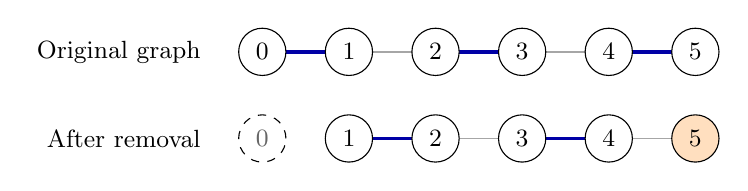
\begin{tikzpicture}[
  x=11mm,y=11mm,font=\small,
  vertex/.style={circle,draw,fill=white,minimum size=6mm,inner sep=1pt},
  path edge/.style={draw=black!35,semithick},
  pair edge/.style={draw=blue!65!black,line width=1.4pt}
]
\node[anchor=east] at (-0.6,0) {Original graph};
\node[anchor=east] at (-0.6,-1) {After removal};
\foreach \row in {0,-1} {
  \foreach \i in {1,...,4} {
    \draw[path edge] (\i,\row) -- ++(1,0);
  }
}
\draw[pair edge] (0,0) -- (1,0);
\draw[pair edge] (2,0) -- (3,0);
\draw[pair edge] (4,0) -- (5,0);
\draw[pair edge] (1,-1) -- (2,-1);
\draw[pair edge] (3,-1) -- (4,-1);
\foreach \i in {0,...,5} {
  \node[vertex] at (\i,0) {\i};
}
\node[vertex,dashed,text=black!60] at (0,-1) {0};
\foreach \i in {1,...,4} {
  \node[vertex] at (\i,-1) {\i};
}
\node[vertex,fill=orange!25] at (5,-1) {5};
\end{tikzpicture}

\caption[Occurrence-capped sampling before and after node removal]{Regenerated subgraphs on the six-node path. Thick blue edges form SCS pairs. Thin grey edges are unselected path edges. The orange node is the BES singleton, and the dashed outline marks the removed node.}
\label{fig:floor1-removal}
\end{figure}

On the original graph, accepting $\{0,1\}$ exhausts the allowance of both nodes. The next available starts are 2 and then 4. After removing 0, the first start is 1 and its only available neighbour is 2. This leaves 3 to pair with 4, and BES takes the remaining singleton $\{5\}$.

Node 0 appears only once on the original graph. Yet the equal-sized containers have no identical items when matched by original node identities and induced edges. Even an optimal matching requires three replacements, including the two original subgraphs that exclude node 0. Both containers are fixed in this construction, so coupling the sampler randomness cannot reduce the discrepancy. The occurrence cap holds on each graph, while the claimed bound of $M$ replacements fails.

A second audit example checks the effect on actual clipped gradients. At fixed model parameters, the directed-path construction with $n=2$, $M=1$, $B=16$, and $C=3$ yields a Euclidean difference of approximately $48$ between the two clipped gradient sums. This exceeds both $CM=3$ and $2CM=6$ for the audited query. Allowing up to $2C$ per changed term accounts for replacement, but using $M$ to count those terms still fails in this example. The witness concerns the audited construction and update. The final-model guarantee for the original caps $(4,10,100)$ remains unestablished, and determining whether that configuration exceeds its targets would require a separate analysis \cite{floor1audit}.

\subsection{Choice of mechanism}
The three-graph sensitivity panel contains 180 newly trained and evaluated runs of Occurrence-Capped PrivIM. The separate six-graph archive records 30 checkpoints from five runs per graph and three budget-group evaluation rows per checkpoint. The later Bitcoin and Facebook step-size study includes 20 runs of this alternative. The audit and the later study record matching source digests for the sampler, accountant, and training entry point. Source equivalence between the audit and the earlier runs remains unverified \cite{floor1audit,floor1runs}.

Both implementations inherit PrivIM's SCS and BES sampling. Occurrence-Capped PrivIM directly extends the original sampler's frequency threshold. PDP-PrivIM runs the inherited sampler inside a redesigned training mechanism. Table~\ref{tab:floor1-comparison} compares the two designs.

\begin{table}[H]
\centering
\caption{Personalization and sensitivity in the two PrivIM-based designs}
\label{tab:floor1-comparison}
\begin{tabularx}{\textwidth}{@{}p{.19\textwidth}XX@{}}
\toprule
Design element & Occurrence-Capped PrivIM & PDP-PrivIM \\
\midrule
Use of targets & Three node occurrence caps & One-time retention, with targets 2 and 4 sharing the base bound \\
Sampling state & One container with shared SCS/BES counts & Separate state in fixed public slots \\
Clipping & Individual subgraph gradients & Individual gradients and each slot sum \\
Node removal & Cross-graph stability remains unestablished & At most two slot contributions can change under the locality assumptions \\
\bottomrule
\end{tabularx}
\end{table}

PDP-PrivIM distinguishes privacy groups through one-time participation. Targets 2 and 4 share the same participation probability and base privacy bound. The sensitivity argument instead relies on a fixed public slot assignment and clipping of whole slot contributions. Under Section~\ref{sec:conditions}, at most two slots can change on node removal, even if every subgraph within those slots changes. Lemma~\ref{lem:sensitivity} bounds the resulting displacement by $2CK=12$. This bound supports the Gaussian accounting and subsequent personalized amplification used for the single-model guarantee in this dissertation.

\section{Locality and sensitivity}
Figure~\ref{fig:pdp-slot-locality} illustrates locality after participation. At a fixed past noisy transcript, the two slots that exclude $v$ receive identical local graphs on both sides, so their contributions agree under the same local role streams.

\begin{figure}[!htbp]
\centering
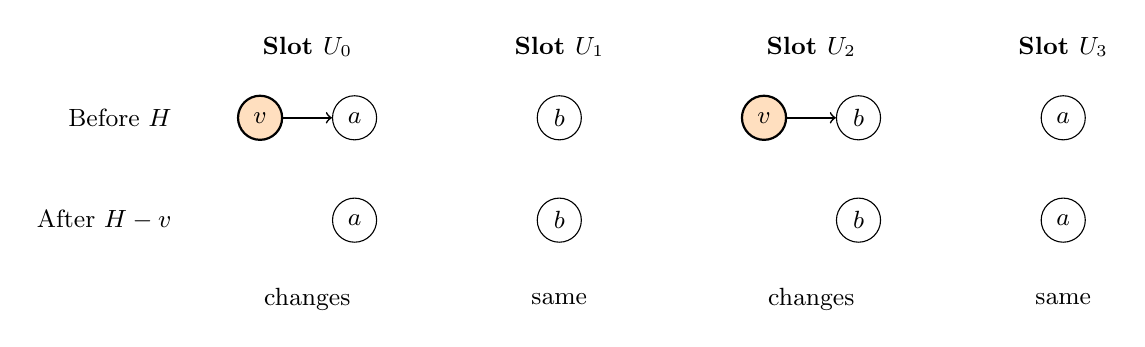
\begin{tikzpicture}[
  font=\small, x=1mm, y=1mm,
  vertex/.style={circle, draw, inner sep=1pt, minimum size=5.6mm, fill=white},
  removed/.style={vertex, thick, fill=orange!25},
  edge/.style={semithick, ->}
]
\foreach \x/\slot/\name in {0/0/changes,32/1/same,64/2/changes,96/3/same} {
  \node[font=\small\bfseries] at (\x,0) {Slot \(U_{\slot}\)};
  \node at (\x,-32) {\name};
}
\node[anchor=east] at (-16,-9) {Before \(H\)};
\node[anchor=east] at (-16,-22) {After \(H-v\)};

\node[removed] (v0) at (-6,-9) {\(v\)};
\node[vertex] (a0) at (6,-9) {\(a\)};
\draw[edge] (v0) -- (a0);
\node[vertex] at (6,-22) {\(a\)};

\foreach \y in {-9,-22} {
  \node[vertex] at (32,\y) {\(b\)};
  \node[vertex] at (96,\y) {\(a\)};
}

\node[removed] (v2) at (58,-9) {\(v\)};
\node[vertex] (b2) at (70,-9) {\(b\)};
\draw[edge] (v2) -- (b2);
\node[vertex] at (70,-22) {\(b\)};
\end{tikzpicture}

\caption[Node removal under stable slot assignment]{Node removal under stable slot assignment. In this illustrative retained graph, $v$ belongs to $U_0$ and $U_2$. Removing $v$ deletes its incident edges and can change computations only in those two slots. The slot assignments of $a$ and $b$ stay fixed.}
\label{fig:pdp-slot-locality}
\end{figure}

\begin{lemma}[Conditional slot-sum sensitivity]\label{lem:sensitivity}
For any fixed data-independent non-Gaussian role tape and common past noisy transcript, node add/remove adjacency changes $S_t$ by at most $2CK=12$ in Euclidean norm.
\end{lemma}
\begin{proof}
Fix the public initialization and the same history $h_t=(Y_0,\ldots,Y_{t-1})$ on both inputs. The current parameters are the same function of that history. If $v\notin U_j$, deleting $v$ leaves the entire induced slot graph unchanged. Stable local ordering, its independent sampling and batch streams, and the slot's cache and cursor are therefore unchanged by induction. Its bounded contribution agrees on both sides.

At most two slots contain $v$. Within those slots, node deletion may change every sampled position, random consumption, walk transition, or cache entry. No finer stability is assumed. Each final slot vector lies in a radius-$C$ ball, so
\begin{equation}
 \|S_t(G;h_t)-S_t(G-v;h_t)\|_2
 \leq\sum_{j:v\in U_j}\bigl(\|b_{tj}(G)\|_2+\|b_{tj}(G-v)\|_2\bigr)
 \leq 2CK=12.
\end{equation}
Changing public $n$ or $M$ can change all samples in an affected slot. The same sensitivity bound holds as long as slot membership and local sampling satisfy Section~\ref{sec:conditions}, the fixed four-by-four padding rule is preserved, and each slot contribution is clipped to $C=3$. The SCS threshold $M$ controls within-slot sampling; the public slot assignment fixes $K=2$. Separately, $\|S_t\|_2\leq4C=12$ by the triangle inequality.
\end{proof}

\subsection{Clipping and padding as parts of the query}
Clipping at the two levels addresses different features of the computation. At the position level, each of the up to four gradient vectors in a slot enters the sum with a bounded norm, and a missing vector is zero. At the slot level, the entire sum is mapped into the radius-$C$ ball before aggregation. The proof tolerates complete replacement of that slot sum. For comparison, with only position clipping, the sum of four bounded vectors can have norm $4C$. Bounding two changed slot sums by their radii would then give the weaker generic sensitivity bound $2K(4C)$, using the same locality argument. Slot clipping replaces $4C$ by $C$ in that calculation. The positional clipping remains relevant to the training direction when a single subgraph gradient would otherwise dominate the sum before slot clipping.

The fixed batch denominator also has a direct role. For the mean-scaled query, dividing by $B=16$ multiplies both the sensitivity bound and the Gaussian standard deviation by the same public factor. A mean normalized by the number of nonempty positions would be a different query. To see the issue, write $m$ and $m'$ for positive, possibly different position counts on adjacent graphs. The difference between normalized signals would decompose as
\begin{equation}
 \frac{S}{m}-\frac{S'}{m'}
 =\frac{S-S'}{m}+
       S'\left(\frac{1}{m}-\frac{1}{m'}\right).
 \label{eq:variable-normalization}
\end{equation}
The second term can change the weight of even the unchanged slots. The stored kernel instead uses the same denominator for empty, partially filled, and full batches. The Gaussian enters on the sum scale, and the fixed scaling of the noisy sum preserves the accounting in the update.

\section{Gaussian RDP and adaptive composition}
For fixed common history, the conditional distributions of $Y_t$ are Gaussians with covariance $\sigma_T^2 I_{2340}$. At any real order $\alpha>1$, their divergence satisfies
\begin{equation}
 D_\alpha(\mathcal N(\mu,\sigma_T^2I)\|\mathcal N(\nu,\sigma_T^2I))
 =\frac{\alpha\|\mu-\nu\|_2^2}{2\sigma_T^2}
 \leq\frac{\alpha(2CK)^2}{2\sigma_T^2}.\label{eq:gaussrdp}
\end{equation}
The same bound holds in reverse. It is uniform over every common history, allowing queries to depend adaptively on previous noisy states. The complete transcript density is the product of conditional densities. Integrating the $\alpha$-moment of its likelihood ratio backwards multiplies the per-step moment bounds, giving the bidirectional RDP upper bound
\begin{equation}
 \rho_T(\alpha)=\frac{T\alpha(2CK)^2}{2\sigma_T^2}
              =\frac{T\alpha\,12^2}{2\sigma_T^2}.\label{eq:rdp}
\end{equation}
Private caches need not have identical posterior distributions conditional on history. The proof compares each complete mechanism under a fixed role tape and uses the uniform history-wise query bound.

If the non-Gaussian tape is itself data-independent random information, its marginalization preserves the uniform RDP bound by joint convexity of $p^\alpha q^{1-\alpha}$. One first bounds each tape-conditioned mechanism and then averages the exponentiated divergence bound. One cannot instead assume private state remains independent after conditioning on a noisy transcript. The actual frozen sampling role streams are public and deterministic, so this extension is not required to supply additional amplification.

The projected update is a function of noisy history. It changes later queries but not the uniform sensitivity argument. Consequently it is legitimate within adaptive composition. This does \emph{not} assert that projected training can be obtained by applying one function only to the final unprojected model.

\section{Conversion and numerical certificates}
The conversion follows Proposition~12 of Canonne et al. \cite{canonne2020}. For $a=e^\epsilon$ and $x\geq0$,
\begin{equation}
 (x-a)_+\leq c_\alpha a^{1-\alpha}x^\alpha,\qquad
 c_\alpha=\frac{(\alpha-1)^{\alpha-1}}{\alpha^\alpha}.
\end{equation}
The maximum ratio occurs at $x=\alpha a/(\alpha-1)$. Substituting the likelihood ratio and integrating bounds the hockey-stick divergence by $c_\alpha\exp((\alpha-1)(\rho_T-\epsilon))$. Applying both directional RDP bounds gives
\begin{equation}
 \epsilon_\alpha=\rho_T(\alpha)
 -\frac{\log\delta+\log\alpha}{\alpha-1}
 +\log\frac{\alpha-1}{\alpha}.\label{eq:conversion}
\end{equation}
The minimum nonnegative bound over the fixed grid $\{1.1,1.2,\ldots,99.9\}$ is valid; the grid need not attain the continuous optimum.

For the PDP-PrivIM reference setting $T=100$, $\sigma_{100}=260$, $\delta_0=10^{-5}$, and order 10.3, the base bound is approximately $\epsilon_0=1.982092738991924$. The archived rational certificate verifies a strict conservative bound below 1.982093. It uses the positive series for $\log x$ with $z=(x-1)/(x+1)$ and a bounded tail:
\begin{equation}
 L_N=2\sum_{k=0}^{N-1}\frac{z^{2k+1}}{2k+1},\qquad
 L_N\leq\log x\leq L_N+\frac{2z^{2N+1}}{(2N+1)(1-z^2)}.
\end{equation}
The stored certificates use exact rational arithmetic at the required orders. They certify inequalities about public constants; they do not certify a Gaussian sampler or prove machine-level privacy.

\section{Personalized amplification}
\begin{theorem}[Single-model conditional ideal PDP]\label{thm:pdp}
Under Section~\ref{sec:conditions}, let $(\epsilon_0,\delta_0)$ be a bidirectional base guarantee for the full $T$-update mechanism before participation amplification. Algorithm~\ref{alg:pdp} satisfies the per-identity bidirectional bounds
\begin{equation}
 \epsilon_v=\log\bigl(1+p_v(e^{\epsilon_0}-1)\bigr),\qquad
 \delta_v=p_v\delta_0.\label{eq:amplified}
\end{equation}
For the reference setting, the approximate bounds are
\begin{align*}
\text{target 1:}\quad &(0.986940353797,\ 2.6894142137\times10^{-6}),\\
\text{targets 2 and 4:}\quad &(1.982092738992,\ 10^{-5}).
\end{align*}
\end{theorem}
\begin{proof}
Fix target identity $v$ and couple the participation decisions of all other identities. Their probabilities remain the same under deletion because the Registry is fixed. Let $Q$ be the output distribution without $v$ and $R$ the distribution with $v$ retained, after integrating the common other-node participation. The uniform base guarantee gives $R(F)\leq aQ(F)+\delta_0$ and $Q(F)\leq aR(F)+\delta_0$, where $a=e^{\epsilon_0}$.

With $v$ present the output law is $P=(1-p)Q+pR$, where $p=p_v$. Thus $P(F)\leq[1+p(a-1)]Q(F)+p\delta_0$. For the reverse direction let $D_*=a(1-p)+p$. From the second base inequality,
$aP(F)\geq D_*Q(F)-p\delta_0$, giving
$Q(F)\leq (a/D_*)P(F)+(p/D_*)\delta_0$.
Since $D_*\geq1$ and $[1+p(a-1)]D_*-a=p(1-p)(a-1)^2\geq0$, the common pair in \eqref{eq:amplified} bounds both directions. The final parameters are a measurable function of the private transcript and public initialization, so they inherit the guarantee. Amplification is applied once to the whole training mechanism.
\end{proof}

Targets 2 and 4 have the same participation probability and base mechanism. Therefore the extra allowance above 2 is unused. This is not a proof error, nor does $1.982/4$ measure exact budget consumption. The bound is sufficient and potentially conservative.

\subsection{Interpreting the target-to-bound curve}
Figure~\ref{fig:target-bound} evaluates Equation~\eqref{eq:amplified} with the reference $\epsilon_0$ and the policy in Equation~\eqref{eq:participation}. For a nominal target $\tau$ between zero and two, substituting the participation probability gives
\begin{equation}
 \epsilon(\tau)=\log\bigl(1+\lambda(e^\tau-1)\bigr),
 \qquad \lambda=\frac{e^{\epsilon_0}-1}{e^2-1}<1 .
 \label{eq:target-curve}
\end{equation}
For $\tau>0$, the argument of the logarithm is strictly less than $e^\tau$. The reference epsilon bound is therefore below the nominal target on this branch. Above two, the cap $p_v\leq1$ fixes $\epsilon(\tau)=\epsilon_0$. The delta bound follows the same participation probability and reaches $\delta_0$ at target two. The policy uses the three marked targets. The continuous curve shows how the same formula behaves between those choices.

\begin{figure}[htbp]
\centering
\begin{tikzpicture}[x=2.1cm,y=1.55cm]
 \draw[->,>=stealth] (0,0) -- (4.35,0)
   node[below right,align=left] {Nominal target\\$\tau$};
 \draw[->,>=stealth] (0,0) -- (0,2.65)
   node[above,align=center] {Certified bound $\epsilon(\tau)$};
 \foreach \x in {1,2,4}
   \draw (\x,0.045) -- (\x,-0.045) node[below] {$\x$};
 \foreach \y in {1,2}
   \draw (0.04,\y) -- (-0.04,\y) node[left] {$\y$};
 \draw[gray,densely dashed] (0,0) -- (2.48,2.48)
   node[above right,black] {$\epsilon=\tau$};
 \draw[very thick,blue!65!black,domain=0:2,samples=70]
   plot (\x,{ln(1+(exp(1.982093)-1)*(exp(\x)-1)/(exp(2)-1))});
 \draw[very thick,blue!65!black] (2,1.982093) -- (4.15,1.982093);
 \foreach \x/\y in {1/0.98694,2/1.982093,4/1.982093} {
   \draw[densely dotted,gray] (\x,0.05) -- (\x,\y);
   \fill[blue!65!black] (\x,\y) circle[radius=1.8pt];
 }
 \node[below,blue!65!black] at (3.08,1.94) {$p_v=1$};
\end{tikzpicture}
\caption[Conditional epsilon bound under the participation policy]{Analytical reference curve for the sufficient epsilon bound. Points mark the nominal targets 1, 2, and 4. The curve uses the conservative reference base value 1.982093.}
\label{fig:target-bound}
\end{figure}

The curve also clarifies what a policy comparison can hold constant. Uniform1 meets the strict target with full retention and stronger base perturbation. PDP-PrivIM instead reduces participation for the strict group and uses the reference base guarantee for the retained graph, before amplification. Both satisfy the declared caps under the ideal assumptions. Conditional adjacency bounds address output distributions. They do not determine whether extra retained edges or weaker base perturbation is more valuable for the learning objective on a particular graph.

\section{Uniform controls and theoretical limitations}\label{sec:uniform-bounds}
The uniform controls use the same sensitivity construction with $p_v=1$ for every identity. At 100 projected updates, Uniform1 uses $\sigma_{100}=486$. The grid value is approximately 0.9986929644 at order 17.8, and its rational certificate verifies $\epsilon<0.998694<1$. Uniform4 uses $\sigma_{100}=139$ and order 6.1, with approximate value 3.99699597485 and a strict certificate below 3.997. Both use $\delta=10^{-5}$ for the complete model.

Applying the theorem to a model release requires verifying the domain, Registry, randomness, and output assumptions. Raw graph preparation, private test evaluation, additional disclosures, finite-precision arithmetic, and error channels require separate analysis.

For independently re-sampled models, basic per-node joint-release composition adds their epsilon and delta bounds. A shared outer retained graph requires composition of the base transcripts before one amplification, rather than repeated free amplification. New run IDs, public seeds, or separate processes do not reset privacy loss. A collection of research models or their evaluations is not asserted to fit within one model's policy budget.
